\RequirePackage[2020-02-02]{latexrelease}
\documentclass[letter,scriptaddress,twocolumn, prl,nofootinbib]{revtex4}

\usepackage{amsmath}%,amssymb} 
\usepackage{makeidx}
\usepackage{amsfonts}
\usepackage[ansinew]{inputenc}
%\usepackage[usenames,dvipsnames]{pstricks}
%\usepackage{subfigure}
\usepackage{epsfig}
\usepackage{float}
%\usepackage{pst-grad} % For gradients
%\usepackage{pst-plot} % For axes
\usepackage[colorlinks,hyperindex]{hyperref}
\hypersetup
{
colorlinks,%
citecolor=black,%
linkcolor=black,%
urlcolor=black,%
}

\setlength\textheight{24.5cm}

% --- Comandos novos ---
\newcommand{\dket}[1]{\left| #1 \right)}
\newcommand{\E}[1]{\frac{\hbar^2 #1 ^2}{2m_0}}
\newcommand{\dbra}[1]{\left( #1 \right|}
\newcommand{\dsubmin}[1]{\left( #1 \right)}
\newcommand{\dbraket}[2]{\left( #1 | #2 \right)}
\newcommand{\dbraketm}[3]{\left( #1 \left| #2 \right| #3 \right)}
\newcommand{\ket}[1]{\left| #1 \right\rangle}
\newcommand{\bra}[1]{\left\langle #1 \right|}
\newcommand{\submin}[1]{\left\langle #1 \right\rangle}
\newcommand{\braket}[2]{\left\langle #1 \right. \left| #2 \right\rangle}
\newcommand{\braketm}[3]{\langle #1 \mid #2 \mid #3 \rangle}
\newcommand{\pinterno}[2]{\left( #1 , #2 \right)}
\newcommand{\comut}[2]{\left[ #1 , #2 \right]} % THE COMUTATOR
\newcommand{\seitz}[2]{\left\{ \, #1 \mid  #2 \, \right\}}
\newcommand{\rep}{\emph{rep} }
\newcommand{\irep}{\emph{irrep} }
\newcommand{\ordem}[1]{\mid #1 \mid}
\newcommand{\op}[1]{\mathbb #1 }
\newcommand{\group}[1]{\mathcal #1 }
\newcommand{\vet}[1]{\mathbf #1 }
\newcommand{\argu}[1]{\left( #1 \right)}
\newcommand{\kp}{\vet{k}\cdot\vet{p}}

\makeindex

%--------------------------------------------------------
\begin{document}

\title{Computational Simulation of the 2d Ising Model}

\author{Alex Roseman}
\author{Adrian Hall}
\date{\today}

\begin{abstract}

\end{abstract}

\maketitle

\begin{figure*}[t]
	\begin{center}
		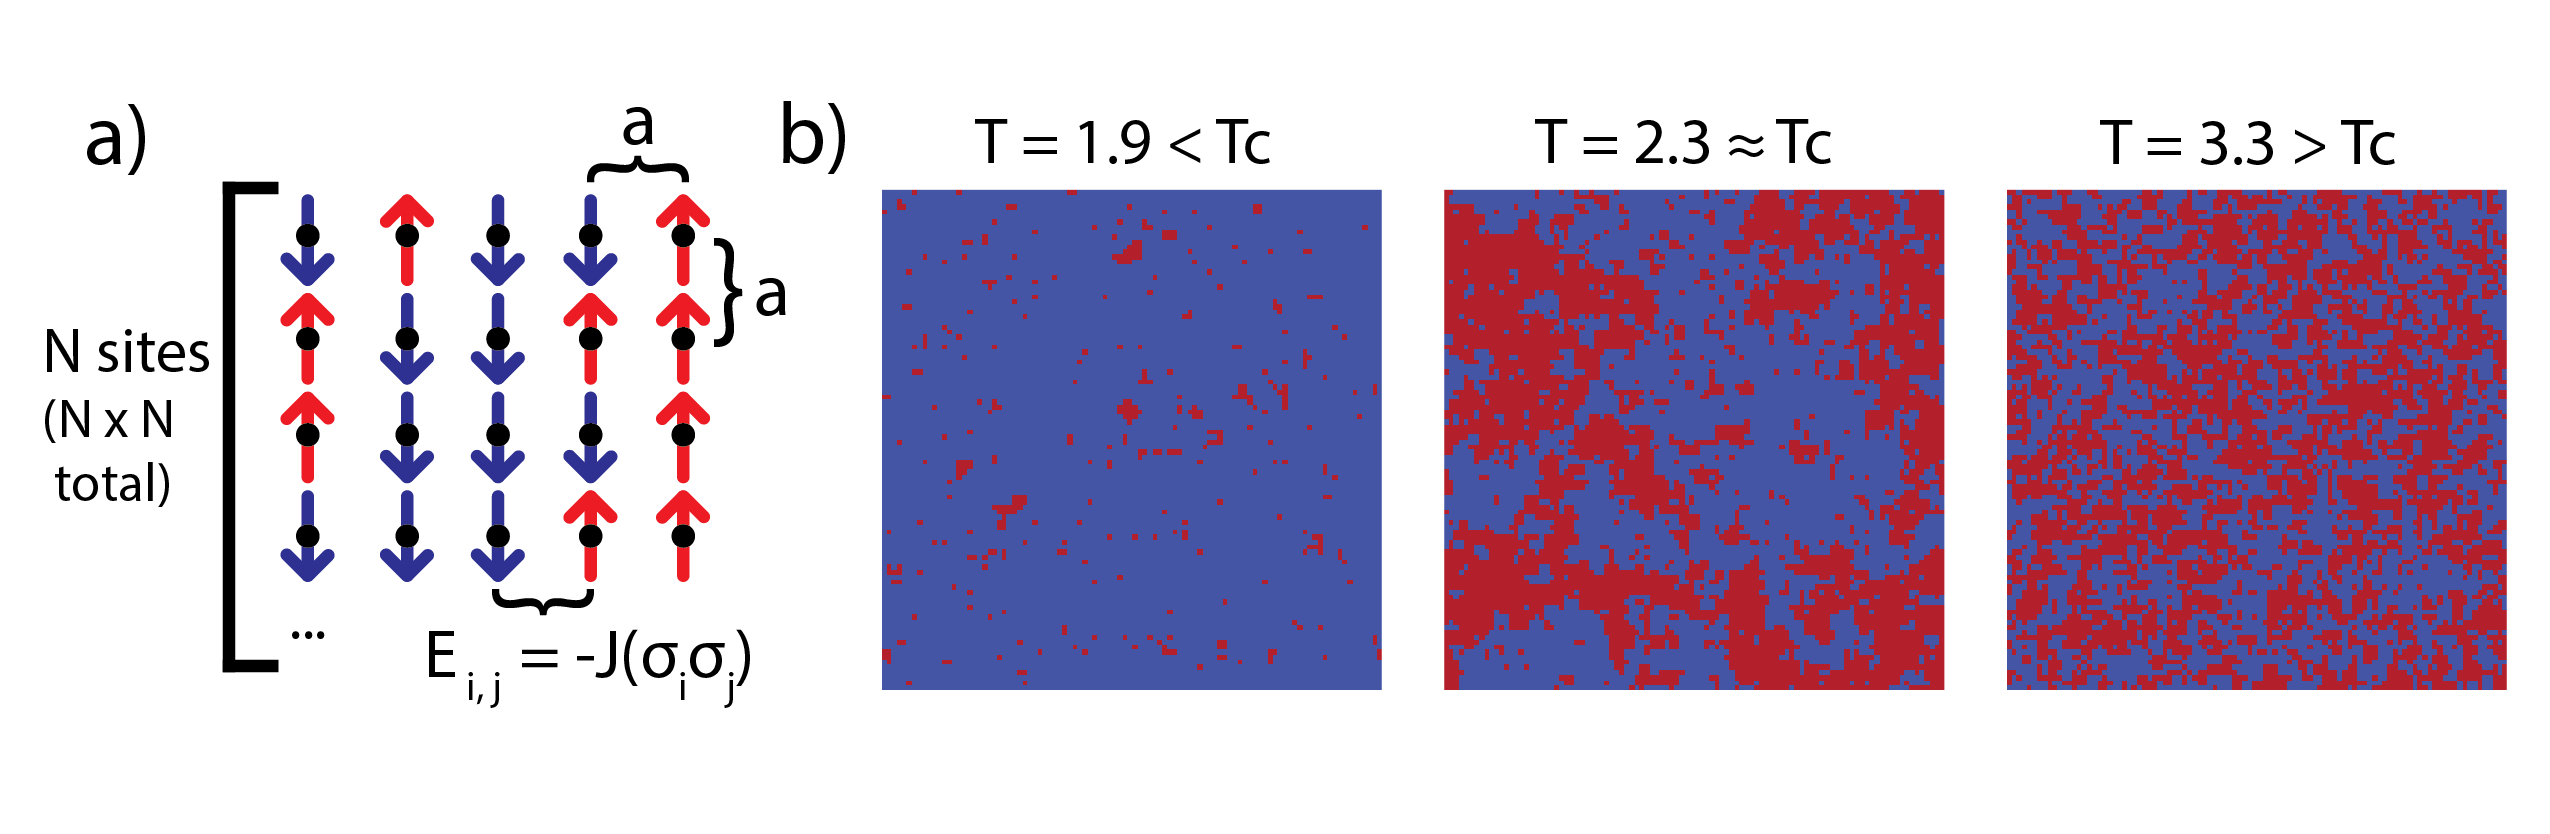
\includegraphics[width=1\textwidth]{figs/fig1.png}
		\caption{a. A diagram of the square lattice. We use lattice size $N = 100$, lattice distance $a = 1$, interaction energy $J = 1$, and spin = $\sigma = \pm 1$ throughout. $E_{i, j}$ is the interaction energy between adjacent spin sites (the lattice wraps around such that each site has 4 neighbors). b. Snapshots after around ten million simulation steps at the given temperature, showing typical states below, near, and above Tc. Red squares have spin up, blue squares spin down.}
		\label{fig:fig1}
	\end{center}
\end{figure*}

\textbf{Introduction:} The Ising model is an idealized model of ferromagnetism and notably one of the few models in statistical mechanics with an exact analytical solution. In the model, a solid material is represented as a regular $d$-dimensional lattice of spin states, each of which can take one of two values ($\pm 1$). The spin states interact with their neighbors and with an external magnetic field according to the Hamiltonian
\begin{equation}
	\label{eq:hamiltonian}
	H = -J \sum_{\langle i, j \rangle} \sigma_i \sigma_j - B \sum_i \sigma_i
\end{equation}
where $\sigma_i$ is the magnetic moment at lattice site $i$, $J$ is the interaction energy, $B$ is the magnetic field strength, and $\langle i, j \rangle$ denotes all pairs of neighboring lattice sites.

Onsager's analytical solution for infinite rectangular lattices \cite{Onsager} describes the equilibrium behavior of the model as a function of $J$ and $B$ as well as the temperature $T$. An interesting feature is that on a lattice that is infinite in two dimensions, the model exhibits a phase transition at the critical temperature $T_c$, given by
\begin{equation}
	\label{eq:Tc}
	\frac{k_B T_c}{J} = \frac{2}{\ln{(1+\sqrt{2})}} \approx 2.269
\end{equation}
where $k_B$ is Boltzmann's constant. At $T_c$ the equilibrium state of the model is discontinuous with respect to temperature. Qualitatively, for $T > T_c$ the lattice is highly disordered, while for $T < T_c$ the spin states correlate significantly with others nearby (\autoref{fig:fig1}).

The model's behavior at temperatures near $T_c$ has been the subject of extensive study. As the temperature approaches $T_c$, several observable quantities vary according to power laws in the reduced temperature $t = \frac{T - T_c}{T_c}$. Among these are specific heat $C_v$, absolute magnetization $|M|$, magnetic susceptibility $\chi$, and correlation length $\xi$. Auto-correlation $\submin{\sigma(0)\sigma(x)}$ also varies according to a power law, although in lattice distance $x$ rather than in $t$. These power laws, and their corresponding exponents (the critical exponents) are not specific to a particular Ising lattice; rather, they are properties of a broader universality class of critical systems \cite{Stanley}. For the Ising model on a rectangular lattice we expect the following behavior near $T_c$: %\autoref{tab:exponents}.

% Table of critical exponents
% \begin{table}[h]
	\begin{center}
		\begin{tabular}{|c|c|c|}
			\hline
			Quantity & Power Law & Predicted Exponent \\
			\hline
			$C_v$ & $|t|^{-\alpha}$ & $\alpha = 0$ \\
			$|M|$ & $|t|^\beta$ & $\beta \approx 1/8$ \\
			$\chi$ & $|t|^{-\gamma}$ & $\gamma \approx 7/4$ \\
			$\xi$ & $|t|^{-\nu}$ & $\nu \approx 1$ \\
			$\submin{\sigma(0)\sigma(x)}$ & $|x|^{-d + 2 - \eta}$ & $ \eta \approx 1/4$ \\
			\hline
		\end{tabular}
%		\caption{Analytical prediction of critical exponents for the $d = 2$ Ising model. All exponents are defined above and below $T_c$ except $\beta$, which is defined only for $T < T_c$. Note that in the case of $\alpha = 0$, the specific heat is expected to diverge logarithmically as $C_v \sim \log t$.}
%		\label{tab:exponents}
	\end{center}
% \end{table}

These critical exponents also obey certain identities [[source?]]:

\begin{equation}
	\text{Rushbrooke's Identity: } \alpha + 2\beta + \gamma = 2 \label{eq:rushbrooke}
\end{equation}
\begin{equation}
	\text{Josephson's Identity: } 2 - \alpha = d * \nu \label{eq:josephson}
\end{equation}
\begin{equation}
	\text{Fisher's Identity: } \gamma = (2 - \eta)\nu \label{eq:fisher}
\end{equation}

\textbf{Methods:} We simulate the 2d Ising Model on an $N$ by $N$ square lattice using the Metropolis-Hastings algorithm, a Markov chain Monte Carlo method which allows random sampling of a state space when only the relative probability of each state is known. We simulate a random walk through the state space of lattice configurations in which each configuration is visited with a frequency proportional to its relative probability, sampled from the Gibbs distribution
\begin{equation}
	P \propto e^{-\frac{E}{k_B T}}
\end{equation}
where $E$ is the energy of the configuration. Throughout the experiment, we use a lattice of size N = 100 with periodic boundary conditions, so that lattice sites 1 and 100 are considered adjacent\footnote{The decision to use N = 100 is explained during analysis of correlation length $\xi$.}. The lattice is initialized to a random configuration, after which the algorithm proceeds as follows. At each step:
\begin{enumerate}
	\item 10\% of lattice sites are selected randomly.
	\item The change in energy $\Delta E_i$ due to flipping the spin of each selected site $i$ is computed according to \autoref{eq:hamiltonian}.
	\item The spin at each selected lattice site is flipped with probability $1$ if $\Delta E_i < 0$, and with probability $e^{-\Delta E_i/(k_BT)}$ otherwise.
\end{enumerate}

In the limit of large numbers of simulation steps, this algorithm faithfully recreates the Gibbs distribution, with a few caveats\footnote{These caveats and the steps taken to mitigate them are described in more detail in Appendix A}.

First, the process must be allowed to converge to the typical set of states. The Metropolis-Hastings algorithm traverses state space at a finite speed, here limited by the $10\%$ of sites considered at each step. However, the initial lattice configuration will not generally be one of high probability; therefore, we must allow sufficient steps for the simulation to arrive at a representative state. We accelerate this process by slowly annealing the lattice, starting with a high temperature ($T_\text{anneal} = 4 \frac{J}{k_B}$) and nonzero external field ($B_\text{anneal} = 0.5 J$). The high temperature discourages the random walk from getting trapped in unfavorable local energy minima, and the external field encourages symmetry breaking at low temperatures where the most favorable configurations are highly magnetized.

Second, lattice configurations in consecutive simulation steps are highly correlated, since each subsequent state is generated by modifying the previous one. This can mean that the sampling uncertainty of the variance in a given quantity will generally be greater than the corresponding mean. We determined that analyzing $200,000$ steps (after achieving convergence) was sufficient to obtain accurate measurements\footnote{See appendix A.}.

\textbf{Data and Analysis:}

We calculate three quantities from the lattice directly. The first is expected energy per lattice site
\begin{equation}
	\label{eq:e_average}
	\submin{E} = \frac{J}{N^2}\sum_{i, j = 1}^{N} \sum_{k} \sigma_{i, j} \sigma_k
\end{equation}
where $\sigma_{i, j}$ is the dimensionless spin of the particle at row $i$, column $j$, and $\sigma_k$ are the spins of its four neighbors. $\submin{E}$ is a straightforward measure of energy, with the number of lattice sites factored out so as not to scale with lattice size (as we are interested in the $N\rightarrow\infty$ limit). For figures, we use a dimensionless $\submin{E}$, with units of $J$.

We calculate a value for $\submin{E}$ over the whole lattice at each simulation step, then extract the mean and standard deviation over the whole simulation at a given temperature (equivalent to an expected value from the Gibbs distribution because the Metropolis-Hastings algorithm spends time in each state proportionate to its probability). In this experiment, we extract the means and standard deviations from one hundred simulation trials, then generate final values for $\submin{E}_T$ by averaging the means from all one hundred simulations at a given temperature together. We use the standard error of this mean to generate uncertainties, considering each simulation a separate measurement.

Similarly, the absolute expected magnetization per lattice site
\begin{equation}
	\label{eq:m_average}
	\submin{M} = \frac{1}{N^2}\sum_{i, j = 1}^{N} \sigma_{i, j}
\end{equation}
where $\sigma_{i, j}$ is the dimensionless spin of particle at row $i$, column $j$. As we take spin and lattice distance to be dimensionless and magnitude one, $\submin{M}$ is unitless. Like $\submin{E}$, it is a straightforward physical measure of magnetization, with the lattice size factored out. As with $\submin{E}$, we calculated expected values over each simulation, then use the mean of these 100 expectation values for final $E$. Uncertainties are calculated as the standard error of this mean. $\submin{E}$ and $\submin{M}$ as functions of $T$ are shown in \autoref{fig:fig2}.

\begin{figure}[h]
	\begin{center}
		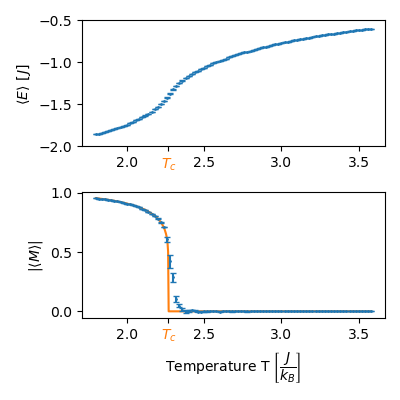
\includegraphics[width=.5\textwidth]{figs/fig2_EMplots.png}
		\caption{Mean energy (top) and absolute magnetization (bottom) per lattice site as computed by MCMC simulation at a range of temperatures. Data is drawn from 100 independent simulations: each data point is the average value of $|M|$ over all simulations; each standard error is the standard error of the mean of $|M|$ over all simulations, treating each $|M|$ as an independent measurement. Analytic $T_c$ (red) and analytic curves for $E$ and $M$ (green) as $N\rightarrow\infty$ are plotted for comparison. At first glance, our system appears to reach phase transition at lower temperature than the analytic $T_c$.}
		\label{fig:fig2}
	\end{center}
\end{figure}

From $\submin{E}$ and $\submin{M}$, we calculate specific heat $c_V$ and magnetic susceptibility $\chi$, using the variance of $E$ and $M$ respectively. It can be shown using the partition function $\mathcal{Z} = \sum_{i} e^{-\frac{E_i}{k_BT}}$ that
\begin{equation}
	\label{eq:cv}
	c_V \equiv \frac{\partial \submin{E_{\text{tot}}}}{\partial T} = \frac{1}{k_BT^2}(\submin{E_{\text{tot}}^2} - \submin{E_{\text{tot}}}^2)
\end{equation}
where $E_{\text{tot}}$ is the total lattice energy. We plot $c_V$ per lattice site, with units of $k_B$. We calculate $c_V$ using the variance of $E$ calculated over simulation steps. As with $\submin{E}$ and $\submin{M}$, we then calculate a final value by averaging over all 100 simulations, and calculate uncertainty as the standard error of this mean.

Similarly, it can be shown that
\begin{equation}
	\label{eq:chi}
	\chi \equiv \frac{\partial \submin{M_{\text{tot}}}}{\partial T} = \frac{1}{k_BT}(\submin{M_{\text{tot}}^2} - \submin{M_{\text{tot}}}^2)
\end{equation}
where $M_{\text{tot}}$ is the total lattice magnetization. Similar to $c_V$, we plot $\chi$ per lattice site, with units of $J^{-1}$. As with $c_V$, we use the variance in $M$ calculated over all lattice steps. As with $\submin{E}$, $\submin{M}$, and $c_V$, we find final values and uncertainties by averaging over multiple simulations.

\begin{figure}[h]
	\begin{center}
		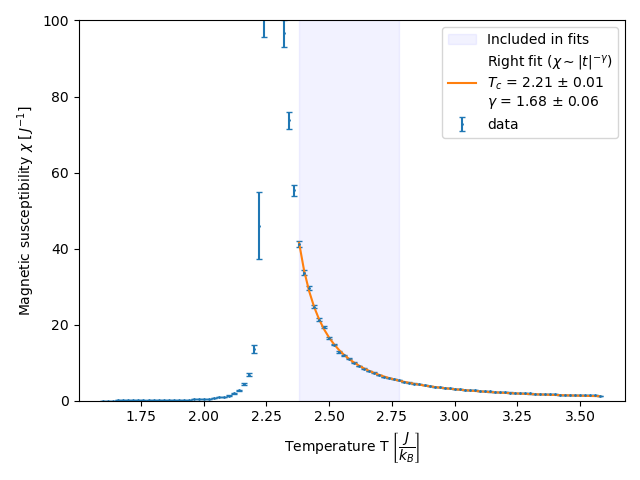
\includegraphics[width=.4\textwidth]{figs/fig3_chi.png}
		\caption{Magnetic susceptibility at a range of temperatures. Susceptibility is calculated from variance in M over each simulation, which is taken as a single measurement. Data points on this graph are the mean of variance(M) over all 97 simulations at a given temperature, and error bars on this graph are the standard error of this mean. Shown in orange is a power law fit with $T_c$ and $\gamma$ considered as free variables, using only the data in the shaded column. NOTE: we intend to merge figures 3 and 4 into a single figure with 2 graphs.}
		\label{fig:fig3a}
	\end{center}
\end{figure}
\begin{figure}[h]
	\begin{center}
		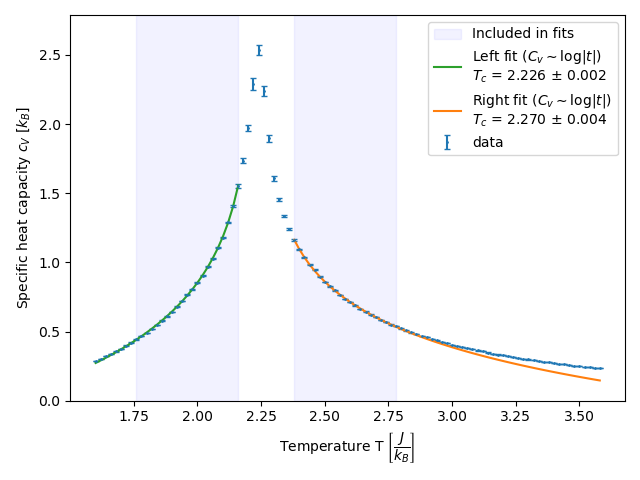
\includegraphics[width=.4\textwidth]{figs/fig3_cv.png}
		\caption{Specific heat at a range of temperatures. Like susceptibility, specific heat is calculated from variance in E across MCMC steps. Data points on this graph are the mean of variance(E) over all 97 independent simulations at a given temperature, and error bars on this graph are the standard error of this mean. Shown in orange and green are logarithmic fits in which $T_c$ was considered a free variable, using only the data in the shaded columns. We generated separate fits on the left and right of Tc. Although the power law should be symmetric, we find significantly different results for Tc. NOTE: we intend to merge figures 3 and 4 into a single figure with 2 graphs.}
		\label{fig:fig3b}
	\end{center}
\end{figure}
\begin{figure}[h]
	\begin{center}
		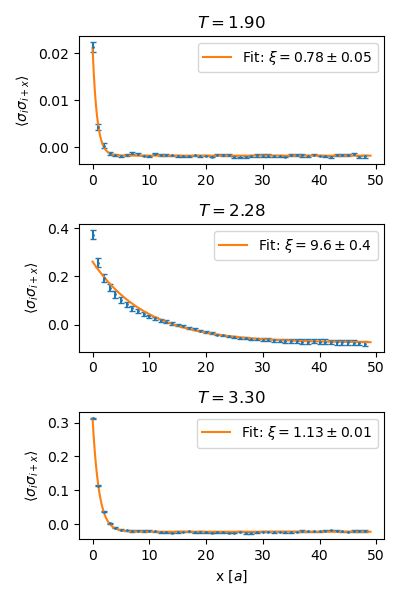
\includegraphics[width=.4\textwidth]{figs/fig4_autocors.png}
		\caption{Autocorrelation functions at representative temperatures: below, near, and above $T_c$. Shown in orange are exponential decay functions fit by least-squares regression to the positive portion of the autocorrelation data, with length scale parameter $\xi$. Autocorrelation seems to become negative (i.e. anticorrelated) after sufficient lattice distance, leading the exponential fit to deviate significantly from the data. This likely plays a role in our terrible estimate for $\nu$. Note: we intend to merge Figs. 5 and 6.}
		\label{fig:fig4a}
	\end{center}
\end{figure}
\begin{figure}[h]
	\begin{center}
		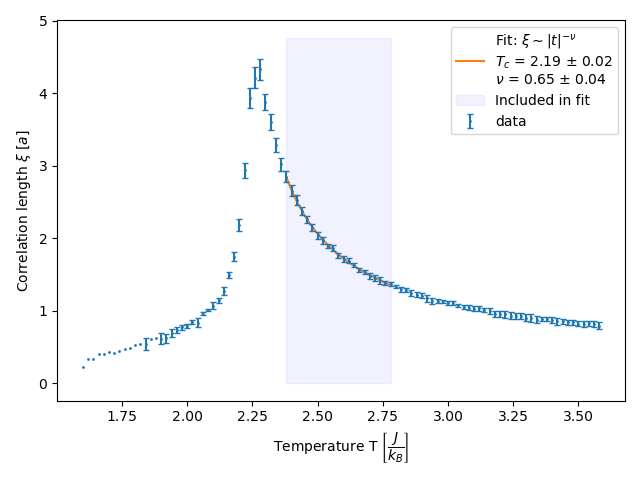
\includegraphics[width=.4\textwidth]{figs/fig4_xi.png}
		\caption{Correlation length $\xi$ at a range of temperatures. These data points are drawn from the fits depicted in Fig. 5, with all the inaccuracy that entails. Uncertainties are drawn from Scipy's curve fit covariance matrix. We intend to include a complete description of the nature of these uncertainties in the body of our report. As with $\chi$ and $c_v$, we fit a power law function (orange) to the data in the shaded region, with $T_c$ and $\nu$ as free parameters. Note: we intend to merge Figs. 5 and 6.}
		\label{fig:fig4b}
	\end{center}
\end{figure}
\begin{figure*}[h]
	\begin{center}
		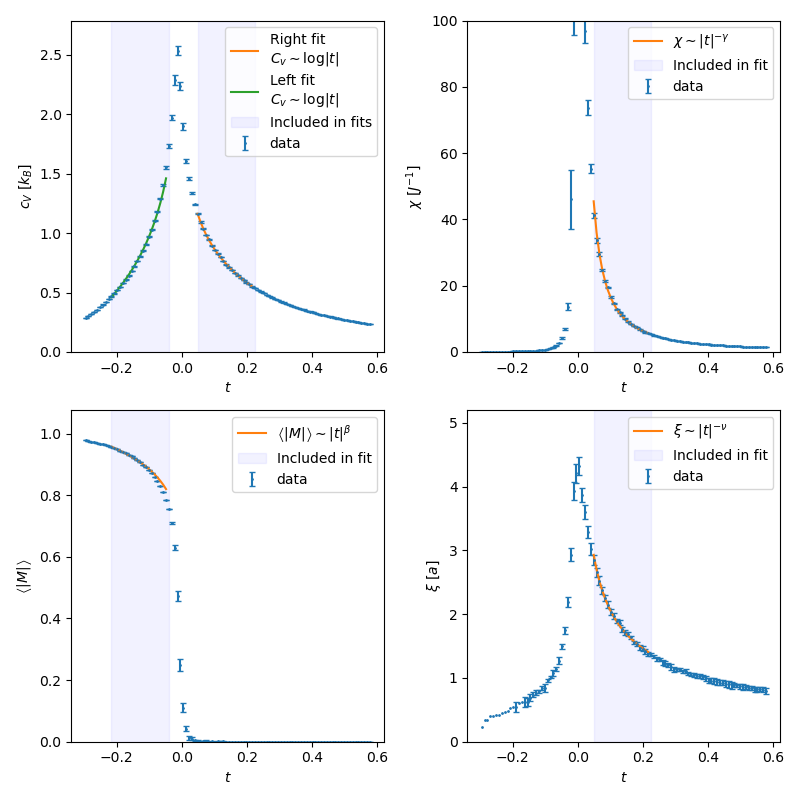
\includegraphics[width=1\textwidth]{figs/fig5_crit_exponents.png}
		\caption{Power law fits for the critical exponents for $c_V$ ($\alpha$) (upper left), $\chi$ ($\gamma$) (upper right), $|M|$ ($\beta$) (lower left), and $\xi$ ($\nu$) (lower right). We attempt to show $\alpha = 0$ by successfully fitting a logarithmic function to $c_V$. In each graph, the x-axis is the normalized temperature $t = \frac{T - T_c}{T_c}$, where $T_c$ is the analytic value of $T_c$. As before, only data from the shaded regions was used for fits. We find the following values: $\gamma = 1.40 \pm .01$, $\beta = 0.103 \pm .002$, $\nu = 0.49 \pm .01$. All critical exponents are, of course, unitless. We have not checked identities because these values are clearly broken, $\nu$ especially (see abstract for details).}
		\label{fig:fig5}
	\end{center}
\end{figure*}

\textbf{Acknowledgements:}
	Prof. Navon, Prof. Newburgh, HongJoon
	
\bibliographystyle{unsrt} 
\bibliography{refs}

\appendix
\section{Appendix A: Convergence}

MOVED FROM METHODS: This process can be sped up via annealing, starting at a high temperature and magnetic field, and then slowly lowering them to the experimental values. The high temperature adds energy to the lattice, lowering the pull of local minima to allow the lattice to find overall lower-energy states. The initial magnetic field breaks the symmetry between positive and negative spin, pulling the lattice away from configurations with large magnetic domains and towards ultimately lower-energy states. As an example, consider a lattice initialized to be split in half down the middle, with the left half spin up, and the right half spin-down. This state is significantly higher-energy than a lattice of all spin up, but reaching the uniform lattice requires passing through less-probably states. At low temperatures, this may not be possible, or might take an arbitrarily large number of steps. Similarly, with no external field, the two large domains might each grow in some places while ceding ground in others. 

Annealing helps prevent these situations. In our simulations, we anneal from $T = 4 J$ and $B = .5 J$, linearly decreasing $T$ and $B$ to the experimental temperature and zero, respectively, over 3,000 steps. We then wait another 5000 steps of "burn-in time," to allow transients from the extra temperature and field to dissipate. This does introduce artifacts into the simulation data: magnetization $M$ is somewhat more likely to be positive than negative, especially at low temperatures. However, this effect is ultimately irrelevant: we use only the magnitude of $M$.

\begin{figure}[h]
	\begin{center}
		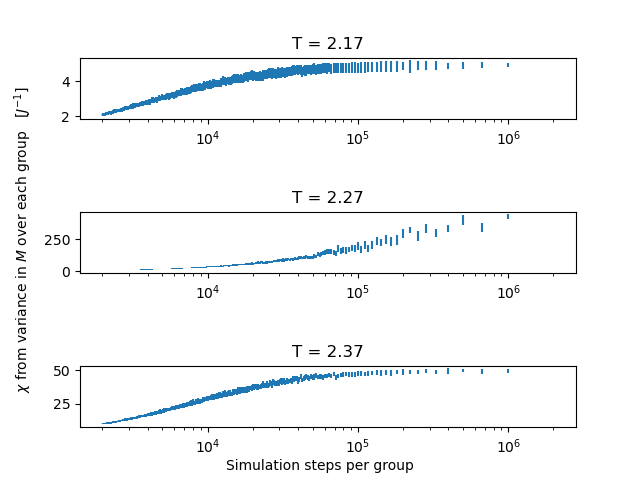
\includegraphics[width=.4\textwidth]{figs/figA1.png}
		\caption{$\chi$ values calculated with data from a simulation of 2,000,000 analyze steps. The total 2,000,000 steps were split as evenly as possible into groups of $n_{steps}$ (x axis), and variance in M was calculated across each group. Each data point is the average variance over all such groups.}
		\label{fig:figA1}
	\end{center}
\end{figure}

\end{document}
